
 \chapter{Competition, Colonization, and Temporal Niche Partitioning}
In this chapter, we will explore and compare models in which transient dynamics at one spatial or temporal scale
result in long-term coexistence at another. All these models assume that
species coexist because there exists at least a brief window in
time during which each species has an advantage. \index{succession}

\begin{figure}[h]
  \centering
  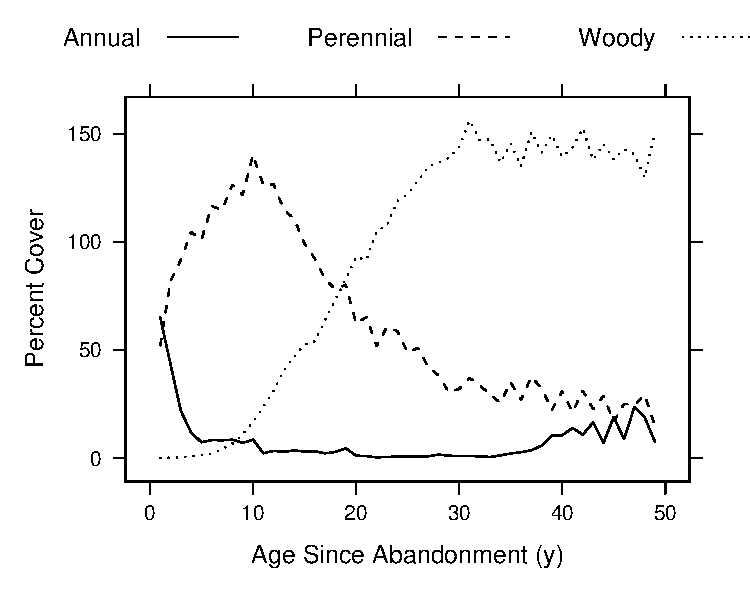
\includegraphics[width=.5\linewidth]{BSsuccFig}
  \caption{Successional trajectory of annual and perennial herbaceous and woody plants in the \index{Buell-Small}Buell-Small Succession Study (http://www.ecostudies.org/bss/). These are mean percent cover from 480 plots across 10 fields, sampled ever 1--2 years.}
  \label{fig:bssucc}
\end{figure}

 We begin with a simple model of the \emph{competition--colonization
   tradeoff}, explore \emph{habitat destruction and the extinction
   debt}, and then examine a model that adds an important subtlety:
 \emph{finite rates of competitive exclusion}. We finish up with an
 introduction to the \emph{storage effect}

\section{\index{competition--colonization tradeoff|see{tradeoffs}}Competition--colonization Tradeoff}
Models of coexistence via this \index{tradeoffs!competition--colonization}tradeoff have been around for awhile \cite{Skellam:1951vn,Levins:1971ve,Horn:1972fk,Armstrong:1976ys, Hastings:1980kx,Shmida1984, Levin:1984uq}. In this tradeoff, species coexist because all individuals die, and therefore all species have to have some ability to colonize new space. Therefore, this means that species have two ways of being successful. Successful species may be very good at colonizing open sites, or they may be very good at displacing other species from a given site. These two extremes setup the basic tradeoff \emph{surface}, wherein species coexist when they make this tradeoff in a manner in which none of them have too superior a combination of both traits. 

Here we provide the two-species model of this phenomenon \cite{Hastings:1980kx}. 
We explored the basis of this model back in our chapter on metapopulation dynamics. Simlarly, here we focus on the case where the state variable is the \emph{proportion of available sites}, rather than $N$. In addition, we extend this to two species using \cite{Hastings:1980kx}. Here we represent the proportion of sites occupied by each of two species,
\begin{align}
  \frac{\D p_1}{\D t} &= c_1p_1\left(1-p_1\right) - m_1p_1   \label{eq:cc1a}\\
  \frac{\D p_2}{\D t} &= c_2p_2\left(1-p_1-p_2\right) - m_2p_2 - c_1p_1p_2   \label{eq:cc2}
\end{align}
where $p_i$ is the proportion of available sites occupied by species $i$, and $c_i$ and $m_i$ are the per capita colonizing and mortality rates of species $i$. Note that $m$ is some combination of inherent senescense plus a background disturbance rate; we will refer to these simply as mortality.

As represented in eq. \ref{eq:cc1a}, species 1 is the superior competitor. The rate of increase in $p_1$ is a function of the per capita colonizing ability times the abundance of species 1 ($c_1p_1$) times the space not already occupied by that species ($1-p_1$). One could estimate $c_1$ by measuring the rate at which an open site is colonized, assuming one would also be able to measure $p_1$. The rate of decrease is merely a density-independent per capita rate $m_1$. 

Eq. \ref{eq:cc2} represents the inferior competitor. The first term includes only space that is unoccupied by \emph{either} species 1 or 2 ($1-p_1-p_2$). Note that species 1 does not have this handicap; rather species 1 can colonize a site occupied by species 2. The second species also has an additional loss term, $c_1p_1p_2$ (eq. \ref{eq:cc2}). This term is the rate at which species 1, the superior competitor, colonizes sites occupied by species 2, \emph{and immediately displaces it}. Note that species 1 is not influenced at all by species 2.

\medskip \noindent
\begin{boxedminipage}{\linewidth}
  {\footnotesize
\paragraph{Competition--colonization tradeoff model} 
Here we implement in \R~a function of ODEs for eqs. \ref{eq:cc1a}, \ref{eq:cc2}.
\begin{Schunk}
\begin{Sinput}
> compcol <- function(t, y, params) {
+     p1 <- y[1]
+     p2 <- y[2]
+     with(as.list(params), {
+         dp1.dt <- c1 * p1 * (1 - p1) - m1 * p1
+         dp2.dt <- c2 * p2 * (1 - p1 - p2) - m2 * p2 - c1 * 
+             p1 * p2
+         return(list(c(dp1.dt, dp2.dt)))
+     })
+ }
\end{Sinput}
\end{Schunk}
}
\end{boxedminipage} \medskip

 At equilibrium, species 1 has the same equilibrium as in the Levins single species metapopulation model.
\begin{align}
  \label{eq:3}
  p_1^*&=1-\frac{m_1}{c_1}
\end{align}
The abundance of species 1 increases with its colonizing ability, and decreases with its mortality rate. 

Species 2 is influenced by species 1 --- how do we know? We see the species 1 appears in the equation for species 2. Let's solve for $p_2^*$ now. 
\begin{align}
  \label{eq:4}
  0 &= c_2p_2\left(1-p_1-p_2\right) - m_2p_2 - c_1p_1p_2\notag\\
  0 &= p_2\left(c_2-c_2p_1 - c_2p_2 - m_2 - c_1p_1\right)\notag\\
  0 &= c_2 - c_2p_1 - c_2p_2 - m_2 - c_1p_1\notag\\
  c_2p_2 &= c_2  - c_2p_1 - m_2 - c_1p_1\notag\\
  p_2^* &= 1  - p_1^* -  \frac{m_2}{c_2} - \frac{c_1}{c_2}p_1^*\\
\end{align}
In addition to the trivial equilibrium ($p_2^*=0$), we see that the nontrivial equilibrium depends on the equilibrium of species 1. This equilibrium makes intuitive sense, in that species 2 cannot occupy sites already occupied by species 1, and like species one is limited by its own mortality and colonization rates ($-m_2/c_2$). It is also reduced by a bit due to those occasions when both species colonize the same site ($(c_1/c_2)p_1$), but only species 1 wins. 

Substituting $p_1^*$ into that equilibrium, we have the following.
\begin{align}
  \label{eq:5}
  p_2^* &= 1  - \left(1-\frac{m_1}{c_1}\right) - \frac{m_2}{c_2} -  \frac{c_1}{c_2} \left(1 - \frac{m_1}{c_1} \right)\\
  p_2^* &= \frac{m_1}{c_1} - \frac{m_2 - m_1 + c_1}{c_2}\label{eq:eq2}
\end{align}
What parallels can you immediately draw between the equilibrium for the two species? The form of the equilibrium is quite similar, but with two additions for species 2. The numerator of the correction term includes its own mortality, just like species 1, but its mortality is adjusted downward (reduced) by the mortality of species 1. Thus the greater the mortality rate of species 1, greater is the opportunity for species 2. This term is also adjusted upward by the colonizing ability of species 1; the greater species 1's colonizing ability, the more frequently it lands on and excludes (immediately) species 2, causing a drop in species 2's equilibrium abundance. In order to focus on the competition--colonization tradeoff, it is common to assume mortality is the same for both species. Tradeoffs with regard to martality may also be quite important, especially if high mortality is correlated with high colonization rate, and negatively correlated with competitive ability.

 If we assume $m_1=m_2$, perhaps to focus entirely on the competition--colonization tradeoff, we can simplify eq. \ref{eq:eq2} further to examine when species 2 can invade (i.e. $p_2^* >0$). Eq. \ref{eq:eq2} can simplify to
\begin{align}
  \label{eq:cc7}
  \frac{m}{c_1} &> \frac{c_1}{c_2}
\end{align}
How can we interpret these? Species 2 can invade if the space not occupied by species 1 ($m/c_1$) is greater the species 1's ability to colonize an open patch faster than species 2 ($c_1/c_2$). An alternative representation ($mc_2 > c_1^2$) shows that species two can persist if mortality is high (but cannot exceed $c_1$), or if species 2's colonization rate is high. That seems fairly restrictive, on the face of it. However, if we assume that species 2 is the better competitor, then this simply specifies how much better it has to be; it also indicates that increasing disturbance (and hence mortality) will enhance the abundance of the species which can recolonize those disturbances.

Thus, this model predicts that these species can coexist, even though one is a superior competitor. Further, it predicts that species 2 will become relatively more abundant as mortality increases.


\subsubsection{Estimating colonization and mortality rates}
Just exactly what corresponds to a ``site'' is not always defined, although site-based models such as these have often been used in a qualitative manner to describe the dynamics plant communities \cite{Hurtt1995, Tilman1994, Pacala1997, Pacala1998}. Indeed, such models could describe systems such as a single field, where a ``site'' is a small spot of ground, sufficient for the establishment of an individual \cite{Tilman1994}. Alternatively, a ``site'' could be an entire field in a large region of mixed successional stages. For the time being, let us continue to focus on a single field as a collection of small plots (e.g., $0.1 \times 0.1$\,m), each of which might hold 1--3 potentially reproductive individuals. There may be several ways to estimate model parameters for these sorts of models \cite{Pacala1998, Tilman1994}, and here we try to estimate $c$ and $m$ directly. Assume that we clear all plants from 100 $0.1 \times 0.1$\,m  plots. In the first year, we find that annuals (e.g., ragweed) showed up in 95 plots, and perennials (e.g. goldenrod) showed up in 60 plots. The following year, we find that 70 of the plots have perennials and 90 plots have annuals. Most plots contain both annuals and perennials.

If we make sufficient assumptions, we could easily estimate $c$ and $m$. Further, in making these assumptions and making estimates, we provide an example that allows one to think critically about the ways in which the assumptions are close to reality or are misleading.   

Let us assume that
\begin{compactenum}
  \item perennials are virtually everywhere in this field ($p\approx1$) and annual seeds are abundant throughout the soil ($p\approx 1$, then $cp \approx c$,
    \item these small plots do not contribute much to the propagule pool, and that they receive all of their propagules from the ubiquitous \emph{rain of propagules} from the surrounding vegetation.
      \item in the first two years, these two species do not interact strongly. 
\end{compactenum}
Clearly these assummptions are wrong, but perhaps not too wrong, and
will allow us to calculate some  back-of-the-envelope estimates of
parameters. With these assumption, we can estimate $c$ and $m$ using
the \emph{propagule rain} \index{metapopulation!propagule rain, estimation}metapopulation model, $\dot{p} = c(1-p) -
mp$. The discrete time version of this is simply the difference equation\footnote{In general, we can create a difference equation from any differential equation, $\dot{N}=F(N)$, where $N_{t+1}=N_t + F(N)$ but where parameter estimates will differ somewhat.}
\begin{equation}
  p_{t+1}= p_t  +c_d(1-p_t)-m_dp_t
  \end{equation}
where $c_d$ and $m_d$ are the discrete time versions of the colonization  and mortality constants. 

With only two parameters, we need only a small amount of data to estimate these constants --- remember the old rule from algebra? We need two equations to estimate two unknowns. Based on our data above, we have
\begin{align*}
  0.5 &= 0 + c_d\left(1-0\right) - m_d\left(0\right)\\
  0.7 &= 0.5 + c_d\left(1-0.5\right) - m_d\left(0.5\right)
\end{align*}
and very quickly we find that $c_d=0.5$ and, given that, we find that $m_d=0.1$.

We have another species as well, and we can estimate $c_d$ and $m_d$ for species 2 as well.
\begin{align*}
  0.95 &= 0 + c_d\left(1-0\right) - m_d\left(0\right)\\
  0.90 &= 0.95 + c_d\left(1-0.95\right) - m_d\left(0.95\right)
\end{align*}
and very quickly we find that $c_d=0.95$ and, given that, we find that $m_d\approx 0.1$.

What do the dynamics look like if we assume no interaction? Both species rise to achieve their equilibria (Fig. \ref{ccnoint}). We have fit the data assuming that the species did not interact, and clearly this is not true, but we have begun the process of thinking critically about what we mean. 

Let us assume that the species start interacting in year 2 --- what would the dynamics look like? The difference equation for species 2 then becomes
\begin{equation}
  \label{eq:ccint2}
    p_{2,t+1}= p_{2,t}  +c_{2,d}(1-p_{2,t})-m_{1,d}p_{2,t} - c_{1,d1}p_{1,t}p_{2,t}
\end{equation}
where we include the subscript for each species. The dynamics differ radically when we include competitive exclusion (Fig. \ref{ccint}). The species reach very different equilibria.
\begin{figure}[ht]
  \centering
  \subfloat[Without interaction]{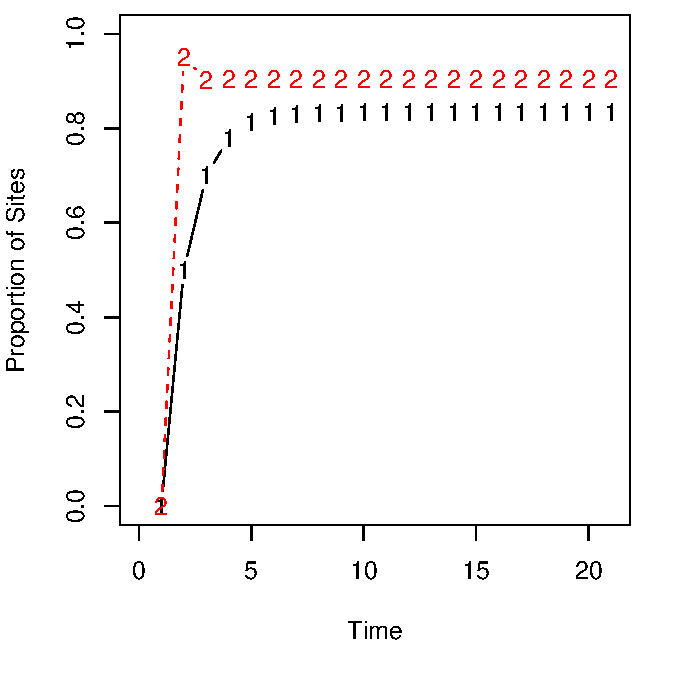
\includegraphics[width=.48\linewidth]{ccnoint} \label{ccnoint}}
  \subfloat[With interaction]{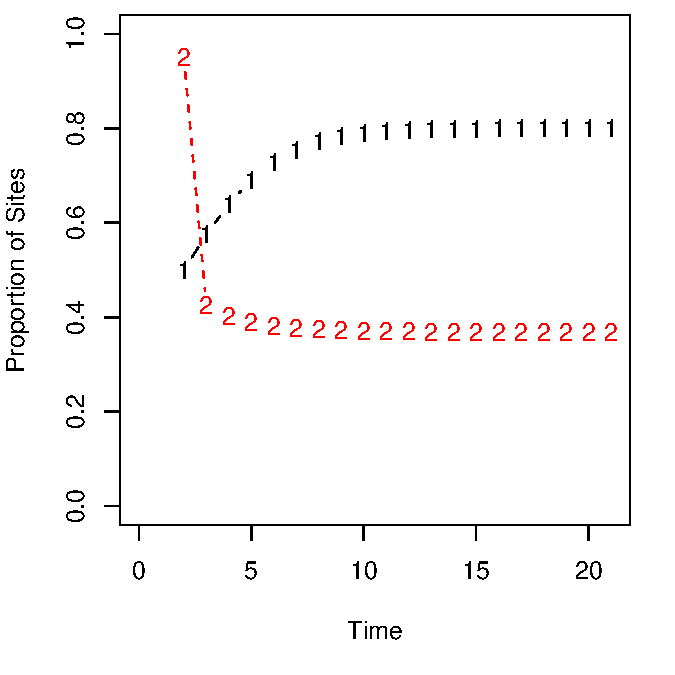
\includegraphics[width=.48\linewidth]{ccint}\label{ccint}}
  \caption{Dynamics of perennials (sp. 1) and annuals (sp. 2) without
    and with interaction. The interaction assumes that species 1
    excludes species 2 instantaneously whenever they come into contact ($c_{d,1}=0.5$, $c_{d,2} = 0.95$,
$m_{d,1} = m_{d,2}= 0.1$)}
  \label{fig:cc}
\end{figure}

Let us extrapolate these dynamics (Fig. \ref{fig:cc}) to secondary succession in general (e.g., Fig. \ref{fig:bssucc}). Our model results seem qualitatively consistent with what we know about successional trajectories. With a lot of open sites, perhaps early in secondary or primary succession, good colonizers get in quickly and fill the site. They are subsequently replaced by the competitively superior species. This is a classic view of \emph{succession}, with \index{pioneer species}pioneer and \index{climax species}climax species. Note that our example focused on small plots within a single field, but we could apply it to a much larger scale. This could approximate a \emph{\index{landscape mosaic}landscape mosaic} composed of patches of different sucessional ages, in which species of different dispersal and competitive abilities persist in the landscape, because they occupy patches of different ages. 


\medskip \noindent
\begin{boxedminipage}{\linewidth}
  {\footnotesize
\paragraph{Estimating and using $c_d$ and $m_d$} 
Let us code the data we derive above, and project over 20 years. First without interaction.
\begin{Schunk}
\begin{Sinput}
> cd1 <- 0.5;  cd2 <- 0.95
> md1 <- 0.1;  md2 <- 0.1
\end{Sinput}
\end{Schunk}
We create a big enough matrix, and perform the projection.
\begin{Schunk}
\begin{Sinput}
> t <- 20
> ps <- matrix(0, nrow = t + 1, ncol = 2)
> for (i in 1:t) ps[i + 1, ] <- {
+     p1 <- ps[i, 1] + cd1 * (1 - ps[i, 1]) - md1 * ps[i, 1]
+     p2 <- ps[i, 2] + cd2 * (1 - ps[i, 2]) - md2 * ps[i, 2]
+     c(p1, p2)
+ }
> matplot(0:t + 1, ps, type = "b", ylab = "Proportion of Sites", 
+     xlab = "Time", xlim = c(0, t + 1), ylim = c(0, 1))
\end{Sinput}
\end{Schunk}
Now assume they interact from year 2 onward.
\begin{Schunk}
\begin{Sinput}
> ps2 <- matrix(0, nrow = t + 1, ncol = 2)
> ps2[1, ] <- ps[2, ]
> for (i in 1:t) ps2[i + 1, ] <- {
+     p1 <- ps2[i, 1] + cd1 * ps2[i, 1] * (1 - ps2[i, 1]) - 
+         md1 * ps2[i, 1]
+     p2 <- ps2[i, 2] + cd2 * ps2[i, 2] * (1 - ps2[i, 2]) - 
+         md2 * ps2[i, 2] - cd1 * ps2[i, 2]
+     c(p1, p2)
+ }
> matplot(1:t + 1, ps2[-(t + 1), ], type = "b", ylab = "Proportion of 
+     Sites", xlab = "Time", xlim = c(0, t + 1), ylim = c(0, 1))
\end{Sinput}
\end{Schunk}
}
\end{boxedminipage} \medskip

\subsubsection{\index{habitat destruction}Habitat destruction}
Nee and May \cite{Nee:1992vn} later showed that, given these tradeoffs, an interesting phenomenon arose. If species coexist via this competition--colonization tradeoff, destruction of habitat increases the abundance of the \emph{inferior competitor}. How does it do this? First let's derive this analytically, and then consider it from an intuitive point of view.

We can alter the above equations to include habitat destruction, $D$.
\begin{align*}
  \frac{\D p_1}{\D t} &= c_1p_1\left(1-D-p_1\right) - m_1p_1\\
  \frac{\D p_2}{\D t} &= c_2p_2\left(1-D-p_1 - p_2\right) - m_2p_2 - c_1p_1p_2
\end{align*}
We can then solve for the equilibria. 
\begin{align}
  \label{eq:9}
    p_1^*&= 1 - D - \frac{m_1}{c_1}\\   
  p_2^* &= \frac{m_1}{c_1}  - \frac{m_2}{c_2} - \frac{c_1}{c_2}\left(1 - D - \frac{m_1}{c_1}\right)\\
\end{align}
What does this mean to us? First note that habitat destruction has a simple and direct negative effect on the abundance of species 1. For species 2, we see the first two terms are unaltered by habitat destruction. The third and last term represents the proportion of colonization events won by the superior competitor, species 1, and thus depends on the abundance of species 1. Because habitat destruction has a direct negative effect on species 1, this term shows that habitat destruction \emph{can increase the abundance of inferior competitors by negatively affecting the superior competitor}. 

We must also discuss what this does \emph{not} mean. Typically, an ecologist might imagine that \emph{disturbed} habitat favors the better colonizer, by making more sites available for good colonizers, and perhaps creating microhabitat conditions that favor rapid growth (e.g., pulse of high resources). This is different than habitat destruction, which  removes entirely the habitat in question. Imagine a parking lot is replacing a grassland, or suburban sprawl is replacing forest; the habitat is shrinking ---  rather than merely being disturbed --- and this has a negative impact on the better competitor.

\subsubsection{Multispecies competition--colonization tradeoff and habitat destruction}
The work of David Tilman and his colleagues in grassland plant communities at the \index{Cedar Creek Natural History Area}Cedar Creek Natural History Area (a NSF-LTER site) initially tested predictions from the $R^*$ model, and its two-resource version, the resource ratio model \cite{Tilman1982,tilman1988,Wedin1993,Wilson1995}. They found that soil nitrogen was really the only resource for which the dominant plant species (prairie grasses) competed strongly. If this is true, then the single resource $R^*$ model of competition predicted that the best competitor would eliminate the other species, resulting in monocultures of the best competitor. The best competitors were little bluestem and big bluestem (\index{Schizachyrium@\emph{Schizachyrium scoparium}}\emph{Schizachyrium scoparium} and \index{Andropogon@\emph{Andropogon gerardii}}\emph{Andropogon gerardii}), widespread dominants of mixed and tall grass prairies, and $R^*$ predicted that they should exclude everything else. However, they observed that the control plots, although dominated by big and little \index{bluestem}bluestem, were also \emph{the most diverse}. While big and little bluestem did dominate prairies, the high diversity of these communities directly contradicts the \index{R@$R^*$}$R^*$ model of competition.\footnote{For different views see \cite{Craine:2005qy,Tilman:2007yb}.} Another pattern they observed was that weaker competitors colonized and became abundant in abandoned fields sooner than the  the better competitors. It turned out that variation in dispersal abilities might be the key to understanding both of these qualitative patterns \cite{Gross1982,Platt1977,Rabinowitz1981}.

In an effort to understand how bluestem-dominated prairies could maintain high diversity in spite of single resource competition,  Tilman generalized the \cite{Hastings:1980kx} equations to include $n$ species\cite{Tilman1994}.
\begin{align}
  \label{eq:cc10}
  \frac{dp_i}{dt} &= c_ip_i\left(1-\sum_{j=1}^{i}{p_j}\right) - m_ip_i - \left(\sum_{j=1}^{i-1}{c_jp_jp_i}\right)
\end{align}
where the last term describes the negative effect on species $i$ of all species of superior competitive ability.

\medskip \noindent
\begin{boxedminipage}{\linewidth}
  {\footnotesize
\paragraph{Multispecies competition--colonization model} 
Here we create an \R~function for eq. \ref{eq:cc10}.
\begin{Schunk}
\begin{Sinput}
> compcolM <- function(t, y, params) {
+     S <- params[["S"]]
+     D <- params[["D"]]
+     with(params, list(dpi.dt <- sapply(1:S, function(i) {
+         params[["ci"]][i] * y[i] * (1 - D - sum(y[1:i])) - 
+             params[["m"]][i] * y[i] - sum(params[["ci"]][0:(i - 
+             1)] * y[0:(i - 1)] * y[i])
+     })))
+ }
\end{Sinput}
\end{Schunk}
This code seems strange, that is, unlike previous systems of ODEs in
which we wrote each separate equation out. The above code merely
implements the strict hierarchy of eq. \ref{eq:10}, and is inspired by a
similar approach by Roughgarden \cite{Roughgarden1998}. It also allows us to specify, on the fly, the number of species  we want. We also sneak in a parameterization for habitat destruction, $D$, and we will address that later. 
}
\end{boxedminipage} \medskip

One goal was to explain the successional patterns of grasses in his study area, the low nutrient grassland/savanna of Minnesota sand plains. Following early succession, the common perennial prairie grass species seemed to form an abundance hierarchy based on competitive ability: the best competitors were the most abundant, and the worst competitors were least abundant. A caricature of a generic species abundance distribution is the geometric distribution, where each species, with rank $i$ makes up a constant, declining, fraction of the total density of all individuals (see Chapter 10 for more detail).\footnote{The most abundant species has rank equal to 1.} Specifically, the proportional abundance of each species $i$ can be calculated as a function of proportional abundance of the most abundant species, $d$, and the species rank, $i$.
\begin{align}
  \label{eq:cc11}
  p_i&=d(1-d)^{i-1}
\end{align}
Thus if the most abundant species makes up 20\% of the assemblage ($d=0.20$), the second most abundant species makes up 20\% of the remaining 80\%, or $0.2(1-0.2)^1=0.16=16\%$ of the community. Tilman \emph{et al.} \cite{Tilman1994} showed that if all species experience the same loss rate, then species abundances will conform to a geometric distribution when colonization rates conform to this rule
\begin{align}
  \label{eq:col}
  c_i&=\frac{m}{\left(1-d\right)^{2i-1}}
\end{align}

\begin{figure}[ht]
  \centering
\subfloat[Equilibria and colonization rates]{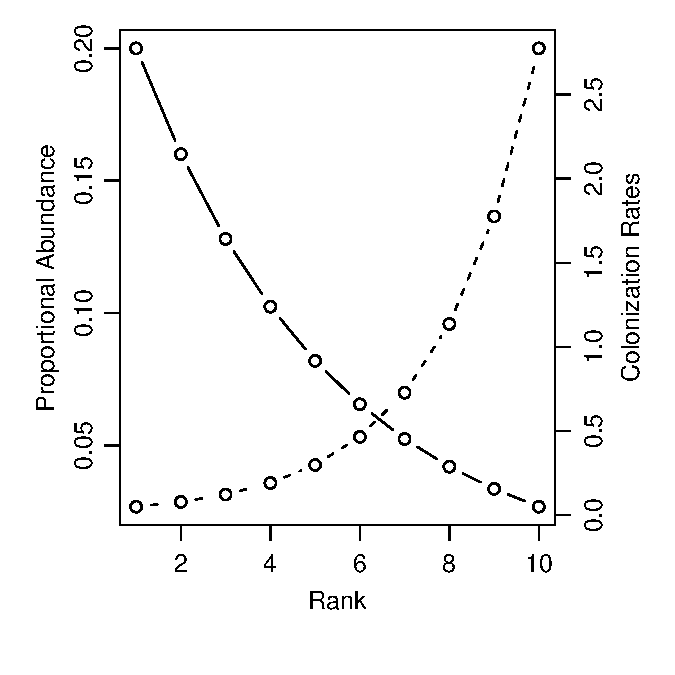
\includegraphics[width=.48\textwidth]{ccM1.pdf}\label{ranks}}
\subfloat[Dynamics]{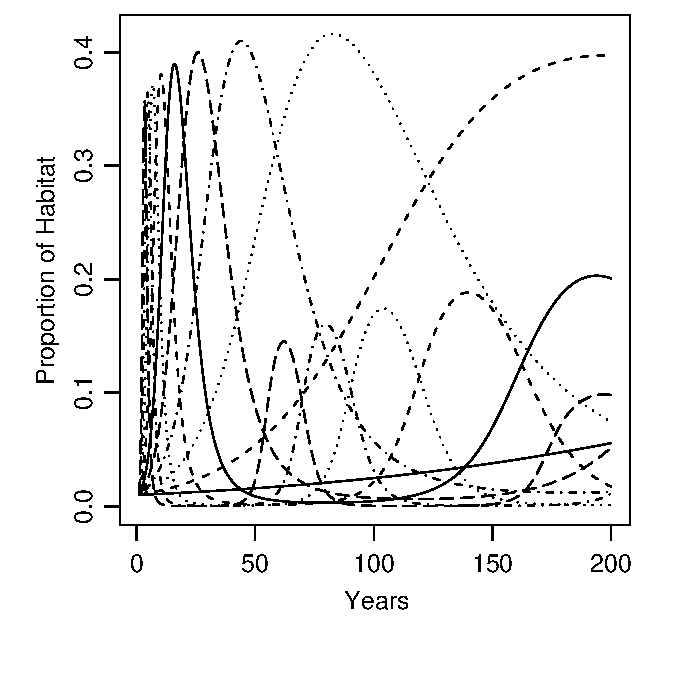
\includegraphics[width=.48\textwidth]{ccM2.pdf} \label{ccdyn}}
  \caption[Equilibrium Properties]{\subref{ranks} Rank--abundance distribution and the colonization rates that create them ($m=0.04$). \subref{ccdyn} Successional dynamics with the competition--colonization tradeoff, from low initial abundances. Here, equilibrium abundance of the best competitor is 20\% ($d=0.2$), mortality is 4\% ($m=0.04$), and colonization rates are determined by eq. \ref{eq:col}, resulting, at equilibrium, in a geometric species rank--abundance distribution.}
\end{figure}


\medskip \noindent
\begin{boxedminipage}{\linewidth}
  {\footnotesize
\paragraph{Calculating  rank--abundance distributions and colonization rates (Fig. \ref{ranks})} 
Here we select 10 species, with the most abundant species equaling 20\% of the biomass in the community, and specify a common mortality or disturbance rate $m$. We then create \emph{expressions} for eqs. \ref{eq:cc11} and \ref{eq:col}.
\begin{Schunk}
\begin{Sinput}
> S <- 10;   ranks <- 1:S
> d <- 0.2;  m = 0.04
> geo.p <- expression(d * (1 - d)^(ranks - 1))
> ci <- expression(m/(1 - d)^(2 * ranks - 1))
\end{Sinput}
\end{Schunk}
Next we create a plot with two $y$-axes.
\begin{Schunk}
\begin{Sinput}
> par(mar = c(5, 4, 1, 4), mgp = c(2, 0.75, 0))
> plot(ranks, eval(geo.p), type = "b", ylab = "Proportional Abundance", 
+     xlab = "Rank", xlim = c(1, S))
> par(new = TRUE)
> plot(ranks, eval(ci), type = "b", axes = FALSE, ann = FALSE, 
+     lty = 2)
> axis(4)
> mtext("Colonization Rates", side = 4, line = 2)
\end{Sinput}
\end{Schunk}
}
\end{boxedminipage} \medskip


\medskip \noindent
\begin{boxedminipage}{\linewidth}
  {\footnotesize
\paragraph{Sucessional dynamics of prairie grasses (Fig. \ref{ccdyn})} 
Here, we set all mortality rates to the same value, one per species, pool all the necessary parameters into a vector (\texttt{params}), and select initial abundances. The initial abundances are merely very low abundances --- this merely results in fun, early successional dynamics.
\begin{Schunk}
\begin{Sinput}
> params <- list(ci = eval(ci), m = rep(m, S), S = S, D = 0)
> init.N <- rep(0.01, S)
> t = seq(1, 200, 0.1)
> cc.out <- ode(init.N, t, compcolM, params)
\end{Sinput}
\end{Schunk}
\begin{Schunk}
\begin{Sinput}
> par(mgp = c(2, 0.75, 0))
> matplot(t, cc.out[, -1], type = "l", ylab = "Proportion of Habitat", 
+     xlab = "Years", col = 1)
\end{Sinput}
\end{Schunk}
}
\end{boxedminipage} \medskip

Tilman and colleagues \cite{Tilman1994b} startled folks when they showed that a common scenario of habitat destruction led to a perfectly counterintuitive result: that habitat destruction led to the very slow but deterministic \emph{loss of the best competitor}. It was unsettling not only that the dominant species would be lost first (a result demonstrated by Nee and May \cite{Nee:1992vn}), but also that the loss of dominant species will take a long time. This implied that we would not realize the true cost of habitat destruction until long after the damage was done. These two conclusions posed a problem for conservationists.
\begin{itemize}
\item Species that were thought safe from extirpation at local scales --- the best competitors --- could actually be the ones most likely to become extinct, and further, 
  \item That the process of extinction may take a long time to play out, and so the data demonstrating this loss might require a long time to collect (Fig. \ref{fig:mhd}).
\end{itemize}
These two predictions constitute the original conception for \emph{\index{extinction debt}extinction debt}. However, the term has become more broadly used to described the latter phenomenon, that extinction due to habitat destruction may take a long time, and current patterns may be a function of past land use \cite{Helm:2006nx,Lindborg:2004gc}.

We see (Fig. \ref{fig:mhd}) the predictable, if counterintuitive, result: the most abundant species, the competitive dominant, becomes extinct over a long period of time, and the next best competitor replaces it as the most abundant species.

\begin{figure}[ht]
\centering
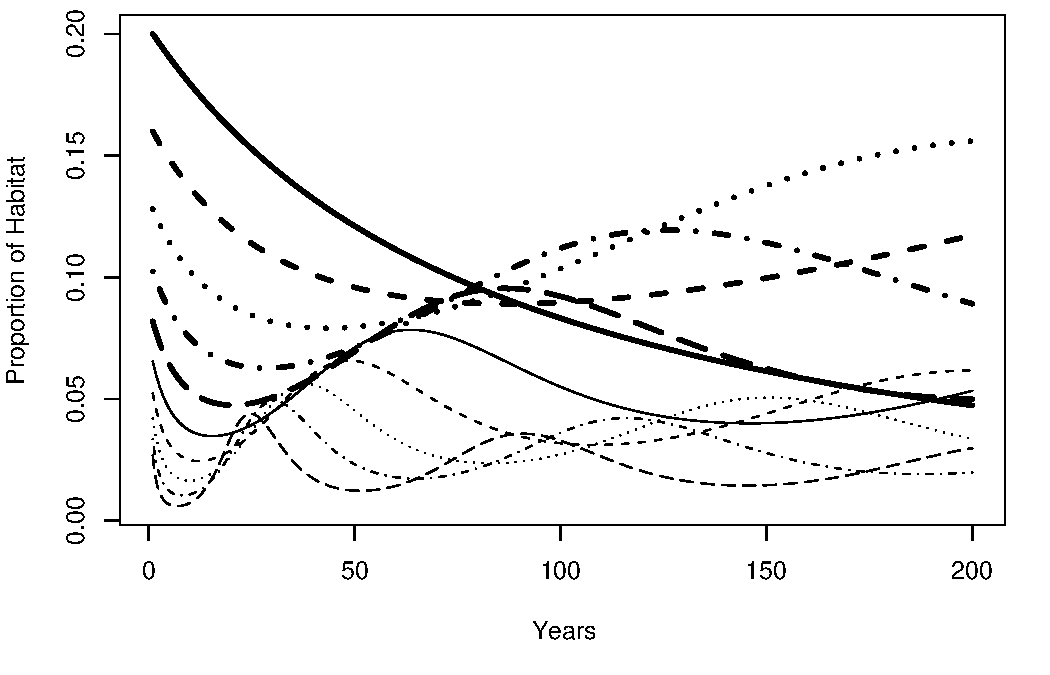
\includegraphics[width=.67\textwidth]{MultiHD.pdf}
\caption{Extinction debt. Destruction of 25\% of the habitat causes the loss of the competitive dominant (wide solid line). Parameters the same as in Fig. \ref{ccdyn}, but initial abundances are equilibrium abundances in the absence of habitat destruction. The second best competitor (wide dashed line) will eventually become the most common species.}
\label{fig:mhd}
\end{figure}

Competition is a local phenomenon, and the better competitor can typically hold onto a given site; however, individuals of \emph{all} species eventually die. Therefore, for two species to actually coexist in a landscape, even the best competitor must colonize some new space at some point. If habitat destruction reduces habitat availability too far, the worst colonizer (i.e., the best competitor) will be unable to disperse effectively to new habitat.


\medskip \noindent
\begin{boxedminipage}{\linewidth}
  {\footnotesize
\paragraph{Extinction debt (Fig. \ref{fig:mhd})} 
We use the same functions and parameters as above. We add habitat destruction for a quarter of the available habitat, which is greater that the equilibrium for the dominant species, and will result in  the slow loss of the dominant species. We also start the species off at their equilibrium abundances, determined by the geometric distribution.
\begin{Schunk}
\begin{Sinput}
> params["D"] <- 0.25
> init.N <- eval(geo.p)
> cchd.out <- ode(init.N, t, compcolM, params)
> matplot(t, cchd.out[, -1], type = "l", lty = 1:5, lwd = rep(c(3, 
+     1), each = 5), col = 1, ylab = "Proportion of Habitat", 
+     xlab = "Years")
\end{Sinput}
\end{Schunk}
}
\end{boxedminipage} \medskip


\section{Adding Reality: Finite Rates of Competitive Exclusion}
While the competition--colonization tradeoff is undoubtedly important, it ignores some fundamental reality that may be very important in explaining patterns and understanding mechanisms. \emph{The models above all assume competitive exclusion is instantaneous}. That assumption may be approximately or qualitatively correct, but on the other hand, it may be misleading. Given the implications of \emph{extinction debt} for conservation, it is important to explore this further. Indeed, Pacala and Rees did so \cite{Pacala1998}, and came to very different conclusions than did Tilman \emph{et al.} \cite{Tilman1994}. This section explores the work of Pacala and Rees \cite{Pacala1998}.

If we look at species in the real world, a couple of observations arise, with respect to tradeoff of species of different successional status. \emph{First}, species characterized by high dispersal ability are also often characterized by high maximum growth rates, related to high metabolic and respiration rates, and allocation to reproductive tissue. These we refer to as \emph{\index{r-selected}r-selected} species \cite{MacArthur1967,MacArthur:1962lr}.  \emph{Second}, we observe that when deaths of individuals free up resources, individuals with high maximum growth rates can take advantage of those high levels of resources to grow quickly and reproduce. \emph{Third}, we observe that the arrival of a propagule of a superior competitor in the vicinity of a poor competitor does not result in the instantaneous draw down of resource levels and exclusion of the poor competitor. Rather, the poor competitor may continue to grow and reproduce even in the presence of the superior competitor \emph{prior to the reduction of resources to equilibrium levels}. It is only over time, and in the absence of disturbance, that better resource competitors will tend to displace individuals with good colonizing ability and high maximum growth rates.\index{tradeoffs!competition--maximum~growth~rate}

Pacala and Rees \cite{Pacala1998} wanted to examine the impact of finite rates of competitive exclusion on the competition--colonization tradeoff. Implicit in this is the role of maximum growth rate as a trait facilitating coexistance in the landscape. High growth rate can allow a species to reproduce prior to resource reduction and competitive exclusion. This creates an ephemaral niche, and Pacala and Rees referred to this as the \emph{\index{successional niche}successional niche}. Species which can take good advantage of the successional niche are thus those with the ability to disperse to, and reproduce in, sites where resources have not yet been depleted by superior competitors. To facilitate their investigation, Pacala and Rees added \emph{\index{finite rate of competitive exclusion}finite rates of succession} to a simple two species competition--colonization model. 

\paragraph{Possible community states} 
They envisioned succession on an open site proceeding via three different pathways. They identified five possible states of the successional community (Fig. \ref{fig:PR}).
\begin{enumerate}
\item \emph{Free} --- Open, unoccupied space.
\item \emph{Early} --- Occupied by only the early sucessional species.
\item \index{susceptible|see{successional niche, SIR models}}\emph{Susceptible} --- Occupied by only the late successional species and susceptible to invasion because resource levels have not yet been driven low enough to exclude early successional species.
\item \emph{Mixed} --- Occupied by both species, and in \emph{transition} to competitive exclsuion.
\item  \index{resistant|see{successional niche, SIR models}}\emph{Resistant} --- Occupied by only the late successional species and resistant to invasion because resource levels have been driven low enough to exclude early successional species.
\end{enumerate}

\paragraph{Pathways}
Given the five states, succession can then proceed along any of three pathways (Fig \ref{fig:PR}):
\begin{enumerate}
\item Free $\rightarrow$ Early $\rightarrow$ Mixed $\rightarrow$ Resistant,
\item Free $\rightarrow$ Susceptible $\rightarrow$ Mixed $\rightarrow$ Resistant,
\item Free $\rightarrow$ Susceptible $\rightarrow$ Resistant.
\end{enumerate}

\begin{figure}[ht]
  \centering
  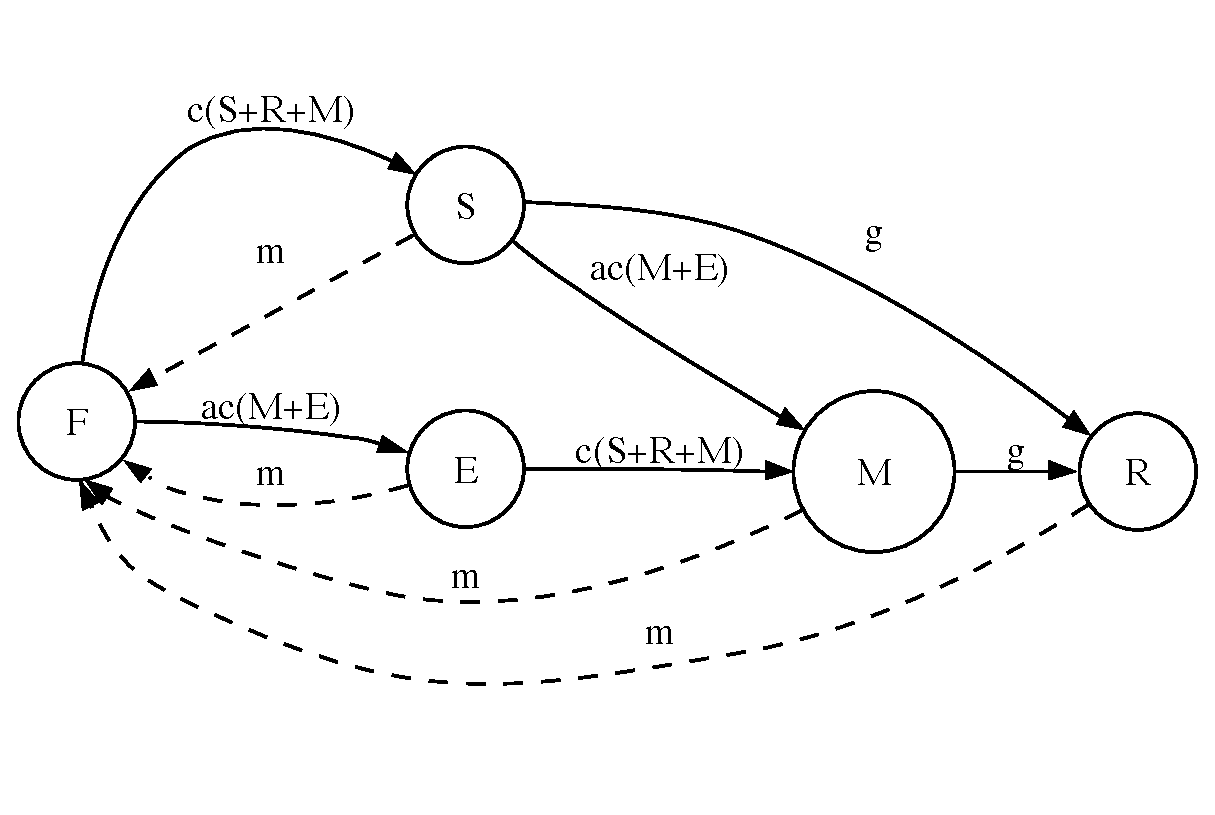
\includegraphics[width=\textwidth]{PandR}
  \caption{The state variables in the \cite{Pacala1998} model. Dashed lines indicate mortality; the larger size of the Mixed state merely reminds us that it contains two species instead of one. Each pathway is labelled with the per capita rate from one state to the other. For instance the rate at which Mixed sites are converted to Resistant sites is $g(M)$, and the rate at which Free sites are converted to Early sites is $ac(M+E)$}
  \label{fig:PR}
\end{figure}

In this context, Pacala and Rees reasoned that the competition--colonization tradeoff focuses on mutually exclusive states, and assumes there are only Free, Early, and Resistant states. In contrast, if species coexist exclusively via the competition--maximum growth rate tradeoff, then we would observe only Free, Mixed, and Resistant states. They showed that these two mechanisms are not mutually exclusive and that the roles of finite rates of competitive exclusion and the successional niche in maintaining diversity had been underestimated.

Note that the interpretation of this model is thus a little different than other models that we have encountered. It is modeling the dynamics of \emph{different community states}. It makes assumptions about species traits, but tracks the frequency of different community states. Technically speaking, any metapopulation model is doing this, but in the contexts we have seen, the states of different patches of the environment were considered to be completely correlated with the abundance of each species modeled. Here we have five different state variables, or possible states, and only two species.

The traits of the two species that create these four states are embedded in this model with four parameters, $c$, $\alpha$, $m$, \index{$\gamma$|see{successional niche, SIR models}}$\gamma$. There is a base colonization rate, $c$, relative colonization rate of the poor competitor, $\alpha$, mortality (or disturbance rate), $m$, and the rate of competitive exclusion, $\gamma$. We could think of $\gamma$ as the rate at which the better competitor can grow and deplete resources within a small patch. We model the community states as follows, using $F$ to indicate a fifth state of Free (unoccupied) space.
\begin{align}
  \label{eq:sn1}
  \frac{dS}{dt}& = \left[ c\left(S+R+M\right)\right]F - \left[\alpha c\left(M+E\right)\right]S - \gamma S - mS\\
 \frac{dE}{dt}& = \left[\alpha c\left(M+E\right)\right]F - \left[ c\left(S+R+M\right)\right]E - mE\\
 \frac{dM}{dt}& = \left[\alpha c\left(M+E\right)\right]S + \left[ c\left(S+R+M\right)\right]E - \gamma M - mM\\
 \frac{dR}{dt}& = \gamma\left( S + M\right) - mR\\
          F&= 1-S-E-M-R
\end{align}


\medskip \noindent
\begin{boxedminipage}{\linewidth}
  {\footnotesize
\paragraph{Successional niche model} 
In addition to representing the original successiona niche model, we can also slip in a parameters for habitat destruction, $D$. As with the above model, habitat destruction $D$ is simply a value between 0--1 that accounts for the proportion of the habitat destroyed. Pacala and Rees \cite{Pacala1998} didn't do that, but we can add it here. We also have to ensure that $F$ cannot be negative.
\begin{Schunk}
\begin{Sinput}
> succniche <- function(t, y, params) {
+     S <- y[1]
+     E <- y[2]
+     M <- y[3]
+     R <- y[4]
+     F <- max(c(0, 1 - params["D"] - S - E - M - R))
+     with(as.list(params), {
+         dS = c * (S + R + M) * F - a * c * (M + E) * S - 
+             g * S - m * S
+         dR = g * (S + M) - m * R
+         dM = a * c * (M + E) * S + c * (S + R + M) * E - 
+             g * M - m * M
+         dE = a * c * (M + E) * F - c * (S + R + M) * E - 
+             m * E
+         return(list(c(dS, dE, dM, dR)))
+     })
+ }
\end{Sinput}
\end{Schunk}

}
\end{boxedminipage} \medskip


Now we can examine the dynamics of this model. When we make the rate of competitive exclusion very high, the model approximates the simple competition--colonization tradeoff  (Fig. \ref{fig:PR})\footnote{When $\gamma=5$, this means that in one year, exclusion will be 99.3\% complete, because it is a pure negative exponential process, where $X_t=X_0e^{\gamma t}$. Similarly, recall our calculation of doubling time, $t=log(X)/r$, where $X$ is the relative size of the population (e.g., 2, if the population doubles); here $r<0$ and time is $< 1$.} The susceptible and mixed states are not apparent, and the better competitor slowly replaces the good colonizer.

\medskip \noindent
\begin{boxedminipage}{\linewidth}
  {\footnotesize
\paragraph{Dynamics of the successional niche model with a high rate of competitive exclusion (Fig. \ref{fig:SPR1})} 
For no particular reason, we pretend that the poor competitor is $7 \times$ as fast at colonizing ($\alpha=7$), and that the rate of competitive exclusion is very high, $\gamma=5$. We assume mortality is low, and there is no habitat destruction.
\begin{Schunk}
\begin{Sinput}
> params.suc <- c(a = 7, c = 0.2, g = 5, m = 0.04, D = 0)
\end{Sinput}
\end{Schunk}
Next we let time be 50\,y, and initial abundances reflect a competitive advantage to the early successional species, and run the model.
\begin{Schunk}
\begin{Sinput}
> t = seq(0, 50, 0.1)
> init.suc <- c(S = 0.01, E = 0.03, M = 0, R = 0)
> ccg.out <- data.frame(ode(init.suc, t, succniche, params.suc))
\end{Sinput}
\end{Schunk}
Last we plot our projections.
\begin{Schunk}
\begin{Sinput}
> matplot(t, ccg.out[, -1], type = "l", ylab = "Relative Frequency", 
+     xlab = "Time", ylim = c(0, 1), col = 1)
> legend("right", colnames(ccg.out)[5:2], lty = 4:1, bty = "n")
\end{Sinput}
\end{Schunk}
}
\end{boxedminipage} \medskip

Now let's slow down competitive exclusion, that is, we will slow the transition from $M$ to $R$. We set  $\gamma$ to be a small number, so that only 10\% of the mixed plots become resistant plots over one year ($\gamma=0.1$). When we slow down competitive exclusion,  we see that we get two phenomena (Fig. \ref{fig:SPR2}). First, we get long term persistance of the mixed state, where we always see a fraction of the habitat occupied by both species. In addition, the fraction of the habitat in the mixed state rises to nearly 40\% of the habitat, because we are mimicking early succession. We go through a phase where both species frequently co-occur, even if this is a tranisitory phase.

\medskip \noindent
\begin{boxedminipage}{\linewidth}
  {\footnotesize
\paragraph{Dynamics of the successional niche model with a low rate of competitive exclusion (Fig. \ref{fig:SPR2})}
Here we slow down the rate of competitive exclusion, and 90\% of the mixed sites stay mixed after a one year interval.
\begin{Schunk}
\begin{Sinput}
> params.suc["g"] <- 0.1
> exp(-0.1)
\end{Sinput}
\begin{Soutput}
[1] 0.9048
\end{Soutput}
\begin{Sinput}
> ccg.out <- data.frame(ode(init.suc, t, succniche, params.suc))
\end{Sinput}
\end{Schunk}
We plot our projections.
\begin{Schunk}
\begin{Sinput}
> matplot(t, ccg.out[, -1], type = "l", ylab = "Relative Frequency", 
+     xlab = "Time", ylim = c(0, 1), col = 1)
\end{Sinput}
\end{Schunk}
}
\end{boxedminipage} \medskip

\begin{figure}[ht]\label{fig:SPR}
  \centering
  \subfloat[$\gamma=5$]{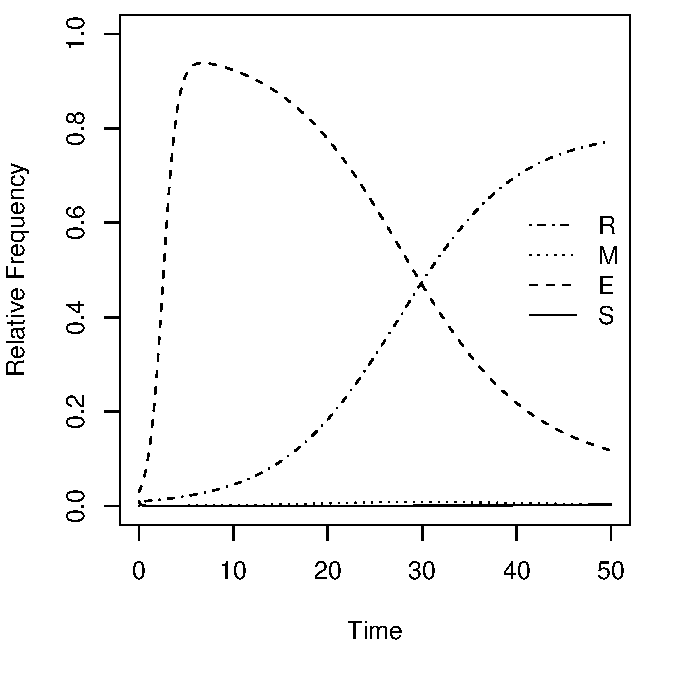
\includegraphics[width=.48\textwidth]{SNPR1}  \label{fig:SPR1}}
  \subfloat[$\gamma=0.1$]{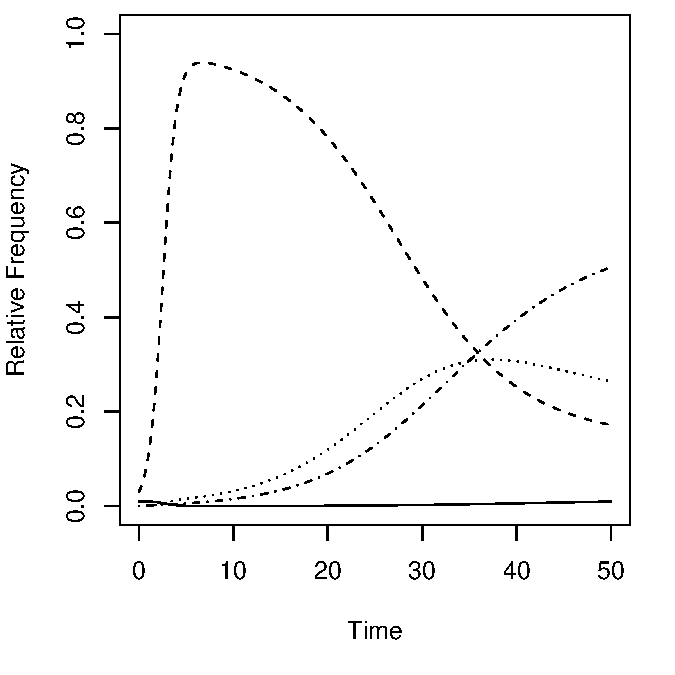
\includegraphics[width=.48\textwidth]{SNPR2}  \label{fig:SPR2}}\\
  \subfloat[$\gamma=0.1,\,m=0.105$]{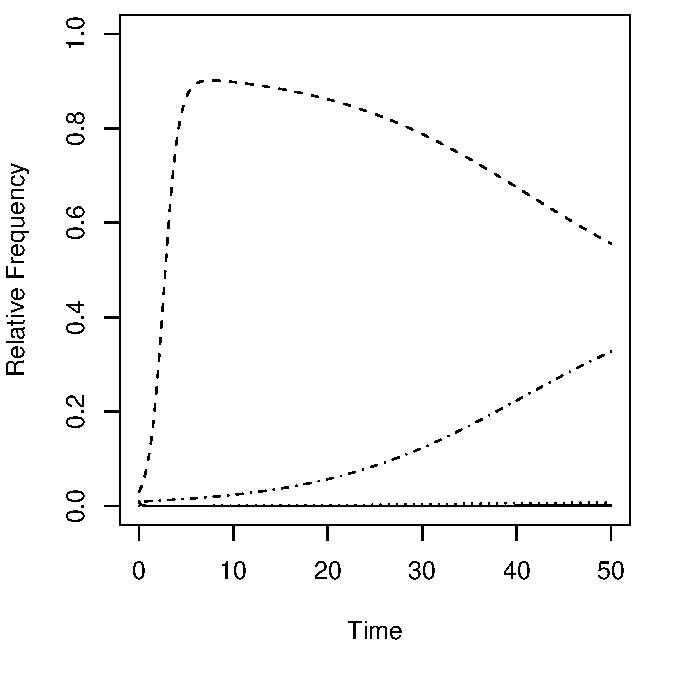
\includegraphics[width=.48\textwidth]{SNPR3}  \label{fig:SPR3}}
  \subfloat[$\alpha=1,\,\gamma=0.1$]{ 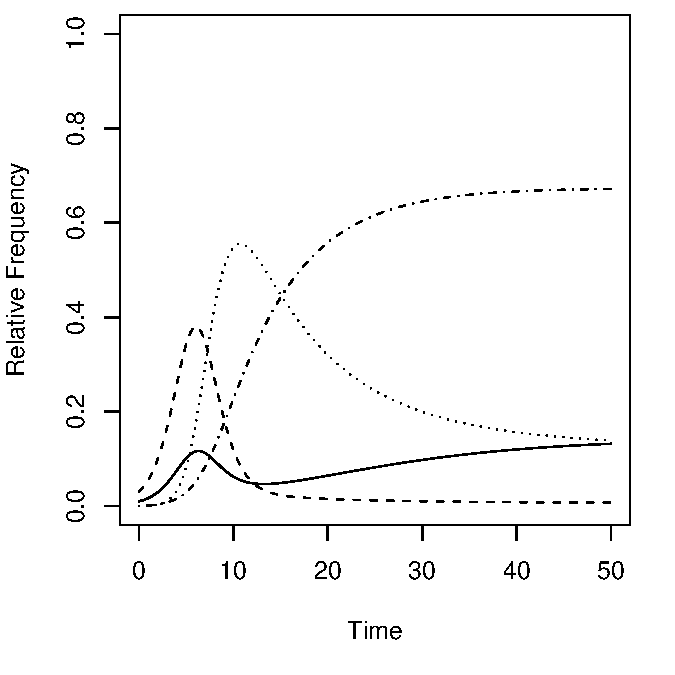
\includegraphics[width=.48\textwidth]{SNPR4}  \label{fig:SPR4}}
  \caption[Dynamics of a successional community]{Unless otherwise noted in the figure, $\alpha=7$, $c=0.7$, $\gamma=5$, $m=0.04$. \subref{fig:SPR1} Competition--colonization (high rate of competitive exclusion),  \subref{fig:SPR2} Competition--colonization and the successional niche (slower competitive exclusion),  \subref{fig:SPR3} Competition--colonization with intermediate disturbance, and \subref{fig:SPR4} Successional niche (equal colonizing ability). }
\end{figure}

Now let's imagine that mortality rates increase, where only 90\% of the habitat remains intact each year ($0.90=e^{-m}$). Even with only a 10\% overall disturbance/mortality rate, the system takes much longer to approach an equilibrium, and has a very high frequency of sites with just the early sucessional species (Fig. \ref{fig:SPR3}).  Where we have moderate disturbance (Fig. \ref{fig:SPR3}), we have greater frequency of the mixed habitat. This reflects the mechanisms underlying the \emph{intermediate disturbance hypothesis} \cite{Connell1978}. At very low disturbance rates, the best competitor prevails. At intermediate disturbance rates, however, we have far more habitat, $M$, that supports both \emph{pioneer} species (good colonizers) as well as \emph{climax} species (superior competitor).

\medskip \noindent
\begin{boxedminipage}{\linewidth}
  {\footnotesize
\paragraph{Dynamics of the successional niche model with an intermediate disturbance rate (Fig. \ref{fig:SPR3})}
Here we have a low rate of competitive exclusion (as above), but higher disturbance rates (10\% of the habitat is disturbed each year).
\begin{Schunk}
\begin{Sinput}
> params.suc["g"] <- 5
> params.suc["m"] <- abs(log(0.9))
> ccg.out <- data.frame(ode(init.suc, t, succniche, params.suc))
> matplot(t, ccg.out[, -1], type = "l", ylab = "Relative Frequency", 
+     xlab = "Time", ylim = c(0, 1), col = 1)
\end{Sinput}
\end{Schunk}
}
\end{boxedminipage} \medskip

Now let's explore the pure successional niche. Imagine that there is no competition--colonization tradeoff: both species have high colonization rates, but the superior competitor retains its competitive edge. However, we also assume that the rate of competitive exclusion is finite ($\gamma \ll \infty$). The pure competition--colonization model would predict that we do not get coexistence. \emph{In contrast, we will find that the successional niche model allows coexistence}. Let's set the relative competitive ability equal ($\alpha=1$) and increase the base colonization rate to the higher of the two original rates ($c=7$). We also let the rate of competitive exclusion be small ($\gamma < 1$). 

What do the dynamics of the pure successional niche model look like (Fig. \ref{fig:SPR4})? We see that we achieve coexistence because the system retains both the mixed state and the resistant state. With both species colonizing everywhere (high $c$), the successional niche allows coexistence because of the finite rate of competitive exclusion. Species 1 now occupies a pure \emph{successional niche} (Fig. \ref{fig:SPR4}).

\medskip \noindent
\begin{boxedminipage}{\linewidth}
  {\footnotesize
\paragraph{Dynamics of the successional niche model with no competition--colonization tradeoff (Fig. \ref{fig:SPR4})}
Here we equal and high colonization rates, and a slow rate of competitive exclusion.
\begin{Schunk}
\begin{Sinput}
> params.suc <- c(a = 1, c = 0.7, g = 0.1, m = 0.04, D = 0)
> ccg.out <- data.frame(ode(init.suc, t, succniche, params.suc))
> matplot(t, ccg.out[, -1], type = "l", ylab = "Relative Frequency", 
+     xlab = "Time", ylim = c(0, 1), col = 1)
\end{Sinput}
\end{Schunk}
}
\end{boxedminipage} \medskip

Let's consider \emph{the successional niche} analytically, by effectively eliminating colonization limitation for either species ($c>>1$, $\alpha=1$). If there is no colonization limitation, then propagules of both species are everywhere, all the time. This means that states $F$, $E$, and $S$ no longer exist, because you never have free space or one species without the other. Therefore $M$ is one of the remaining states. The only monoculture that exists is $R$, because in $R$, both propagules may arrive, but the early successional species 1 cannot establish. Therefore the two states in the pure successional niche model are $M$ and $R$.

How does $M$ now behave? $M$ can only increase when $R$ dies back. $M$ will decrease  through competitive exclusion. We might also imagine that $M$ would decrease through its own mortality; we have stipulated, however, that colonization is not limiting. Therefore, both species are always present, if only as propagules. The rates of change for $M$ and $R$, therefore are,
\begin{align*}
  \frac{\D M}{\D t} &= mR - \gamma M\\
  R &= 1 -M\\
\end{align*}

The equilibria for the two states can be found by first setting $\dot{M}=0$ and substituting $1-M$ in for $R$, as 
\begin{align*}
  0 &= m\left(1-M\right) - \gamma M\\
  M* &= \frac{m}{\gamma + m}
\end{align*}
making $R* = \gamma/(\gamma+m)$. 


Up until now, we have focused on the frequencies of the four \emph{states}, rather than the frequencies of the two types of species (early successional and competitive dominant). If we are interested in the relative abundances of the two types of species, we merely have to make assumptions about how abundant they are in each different state. If we assume that they are equally abundant in each state, then the abundance of the early successional species is $E+M$ and the abundance of the competitive dominant is $S+M+R$.

Let us finally investigate extinction debt with this model. We should first verify that we get extinction debt with a ``pure'' competition--colonization tradeoff (large $\gamma$, large $\alpha$). We should then reduce $\gamma$ and $\alpha$ to make the successional niche the primmary mechanism, and see what happens to the pattern of extinction.


\begin{figure}[ht]
  \centering
  \subfloat[$\alpha=10,\,\gamma=10$]{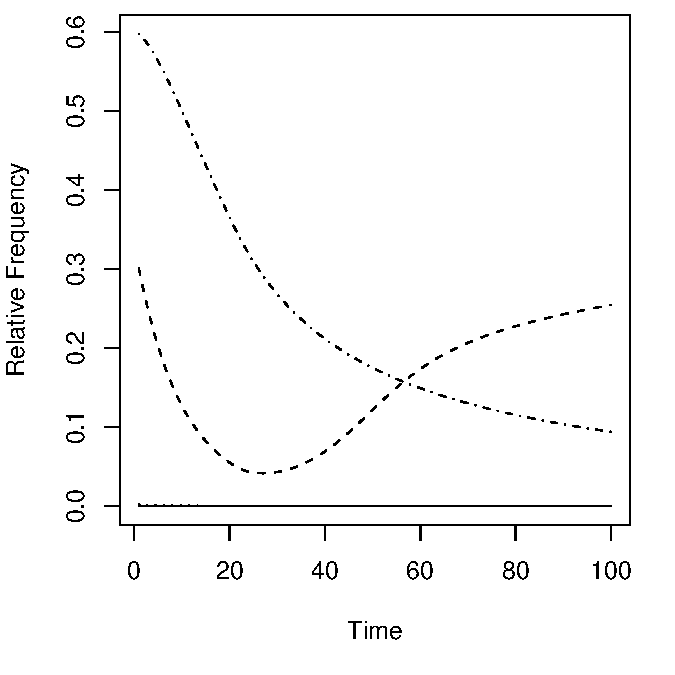
\includegraphics[width=.48\textwidth]{ED1}  \label{fig:ED1}}
  \subfloat[$\alpha=1,\,\gamma=0.1$]{ 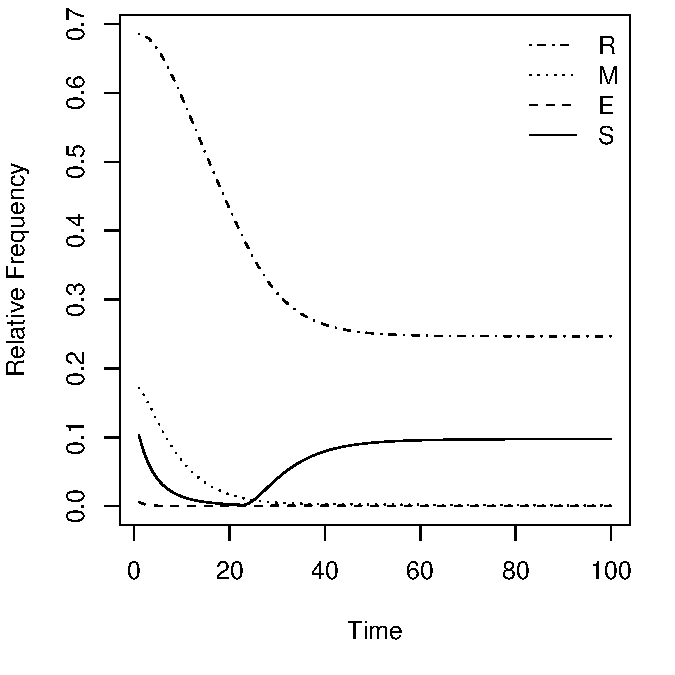
\includegraphics[width=.48\textwidth]{ED2}  \label{fig:ED2}}
  \caption[Dynamics of a successional community]{Extinction dynamics beginning equilibrium abundances. \subref{fig:ED1} Relying on the competition--colonization tradeoff results in a loss of the competitive dominant,  \subref{fig:ED2} Relying on the successional niche tradeoff results in a persistance of the competitive dominant.}
  \label{fig:EDSN}
\end{figure}

We can compare patterns of \index{extinction debt}extinction under these two scenarios (Fig. \ref{fig:EDSN}, without and with the successional niche). In doing so, we find \emph{a complete reversal of our conclusions}: when the primary mechanism of coexistence is the successional niche, we find that the competitive dominant persists, rather than the early successional species. (Recall that when colonization rates are equal, the rate of extinction \emph{must} be slow in order to achieve coexistance even without habitat destruction).

These opposing predictions highlight the important of getting the mechanism right. They also illustrate the power of simplistic models to inform understanding.

\medskip \noindent
\begin{boxedminipage}{\linewidth}
  {\footnotesize
\paragraph{Dynamics of the extinction with the successional niche model (Fig. \ref{fig:EDSN})}
Here we approximate the competitive-colonization model with unequal colonization rates, and a very high rate of competitive exclusion. We then find, through brute force, the equlibria for our parameter set by integrating a long time and keeping the last observations as the equilibria.
\begin{Schunk}
\begin{Sinput}
> params.suc1 <- c(a = 10, c = 0.1, g = 10, m = 0.04, D = 0)
> Xstar1 <- ode(init.suc, 1:500, succniche, params.suc1)[500, 
+     -1]
\end{Sinput}
\end{Schunk}
We then create habitat destruction, and plot the result.
\begin{Schunk}
\begin{Sinput}
> params.suc1D <- c(a = 10, c = 0.1, g = 10, m = 0.04, 
+                   D = as.numeric(Xstar1["R"]))
> t = 1:100
> ccg.out1 <- data.frame(ode(Xstar1, t, succniche, params.suc1D))
> matplot(t, ccg.out1[, -1], type = "l", col = 1, 
+         ylab = "Relative Frequency", xlab = "Time")
\end{Sinput}
\end{Schunk}
Next, we include the successional niche, by making colonization rates equal and high, and $\gamma$ small. We then find our equilibria, without habitat destruction.
\begin{Schunk}
\begin{Sinput}
> params.suc2 <- c(a = 1, c = 1, g = 0.1, m = 0.04, D = 0)
> Xstar2 <- ode(init.suc, 1:500, succniche, params.suc2)[500, 
+     -1]
\end{Sinput}
\end{Schunk}
We then create habitat destruction, and plot the result.
\begin{Schunk}
\begin{Sinput}
> params.suc2D <- c(a = 1, c = 0.7, g = 0.1, m = 0.04, 
+                   D = as.numeric(Xstar1["R"]))
> ccg.out2 <- data.frame(ode(Xstar2, t, succniche, params.suc2D))
> matplot(t, ccg.out2[, -1], type = "l", ylab = "Relative Frequency", 
+     xlab = "Time", col = 1)
> legend("topright", colnames(ccg.out2[5:2]), lty = 4:1, bty = "n")
\end{Sinput}
\end{Schunk}
}
\end{boxedminipage} \medskip

\section{Storage effect}
What if all of this is wrong? What if none of these tradeoffs underlie coexistance? Jim Clark and his colleagues \cite{Clark2004} examined dispersal traits of co-occurring deciduous forest trees (fecundity, dispersal), and  successional status, and found no evidence that early successional species had higher dispersal capacity. This suggests a lack of support for competition--colonization tradeoffs. Rather, they found evidence that \emph{asynchronous success in reproduction} of these \emph{long-lived organisms} allowed them to coexist. Together, these traits constitute a mechanism referred to as the \emph{\index{storage effect}storage effect} \cite{Chesson2000a,Warner1985}.

In the storage effect, competing species can \emph{store} energy for reproduction until favored conditions arise \cite{Chesson2000a,Warner1985}. Assumptions include:
\begin{description}
\item[\textbf{Variable environment}] Each species encounters both favorable and unfavorable periods for reproduction.
\item[\textbf{\index{buffered population growth}Buffered population growth}] Each species stores energy in a resistant stage (e.g., long lived adults, seeds, spores, eggs) between favorable periods.
\item[\textbf{\index{environment--competition covariation}Environment--competition covariation}] The same conditions that favor reproduction for a particular species also increase competition intensity for that species. If, for instance, winter rains favor a particular desert annual, that desert annual will experience the greatest intraspecific competition following a wet winter precisely because of its large population size. 
\end{description}
One prediction of the storage effect is that small population sizes will be more variable (have higher $CV$, coefficient of variation) than large populations of competing species \cite{Kelly2002}. 

In one sense, the storage effect constitutes a temporal niche \cite{Chesson2000a}. That is, the theory simply stipulates that different species succeed at different times. For rare species to coexist with common species, their relative success needs to be somewhat greater than the relative success of common species. In the absence of environmental variability, species would not coexist.

Here we provide one set of equations describing the dynamics of the storage effect for each species $i$ in the community \cite{Chesson:1994pb}.
\begin{gather}
  \label{eq:storage}
  N_{i,t+1} = \left(1-d\right)N_{i,t} + R_{i,t}N_{i,t} \\
  R_{i,t} = e^{E_{i,t} - C_{i,t}} \\
  E_{i,t} = F\left( X_{i,t} \right)\\
  C_{i,t} = \sum_{i=1}^S\alpha_i e^{E_{i,t}}N_{i,t}\\
\end{gather}
Here, $E$ is an unspecified function of the environment, $X_{i,t}$, so that $E$ specifically differs among species and across time. We can think of $exp(E_{i,t})$ (the first growth factor in $R_{i,t}$) as the maximum per capita reproductive rate for species $i$, at time $t$, in the absence of competition. It is determined by the environment at time $t$. 

The other growth factor, $exp(-C_{i,t})$, is the effect of competition. It allows us to intensify competition at large population sizes (e.g., during favorable conditions), and lessen competition at low population sizes (e.g., during poor conditions). These two factors allow us to represent independently the positive and negative effects of the environment on an organism's capacity to grow ($E_i$), and also to represent how competition intensity covaries with population density ($C_i$). There are many other representations of the storage effect  \cite{Chesson2003,Warner1985}, but this is a simple and convenient one \cite{Chesson:1994pb}.

The storage effect is a special case of \emph{\index{lottery models}lottery} models \cite{Morin1999}. Originally developed for reef fishes \cite{Sale1977}, lottery models are considered general models for other systems with important spatial structure such as forest tree assemblages. Conditions associated with lottery systems \cite{Chesson1981} include:
\begin{enumerate}
\item Juveniles (seedlings, larvae) establish territories in suitable locations and hold this territory for the remainder of their lives. Individuals in non-suitable sites do not survive to reproduce.
\item Space is limiting; there are always far more juveniles than available sites.
\item Juveniles are highly dispersed such that their relative abundances and their spatial distributions are independent of the distribution of parents.
\end{enumerate}
These conditions facilitate coexistence because the same amount of open space has a greater benefit for rare species than for common species. While the invulnerable nature of successful establishment slows competitive exclusion, permanent nonequilibrium coexistence does not occur unless there is a storage effect, such as with overlapping generations, where a reproductive stage (resting eggs, seeds, long lived adults) buffers the population during unfavorable environmental conditions, and negative environment--competition covariation.

\subsection{Building a simulation of the storage effect}
Here we simulate one rare and one common species, wherein the rare species persists only via the storage effect. We conclude with a simple function, \texttt{chesson}, that simplifies performing more elaborate simulations.

\paragraph{Fluctuating environment}
First we create a variable environment. Environments are frequently noisy and also temporally autocorrelated --- we refer to a special type of scale-independent autocorrelation as \emph{red noise} or \emph{$1/f$ noise} (``one over 'f' noise'') \cite{Halley1996}. Here we use simply \emph{white noise}, which is not temporally autocorrelated, but rather, completely random at the time scale we are examining.
\begin{Schunk}
\begin{Sinput}
> years <- 100
> t <- 1:years
> variability = 4
> env <- rnorm(years, m = 0, sd = variability)
> plot(t, env, type = "l")
\end{Sinput}
\end{Schunk}
\paragraph{Differential responses to the environment}
A key part of the storage effect is that species have differential reproduction in response to a fluctuating environment  (Fig. \ref{fig:rho}). However, species can differ for all sorts of reasons. Therefore, we will let our two species have different \emph{average} fitness. We do this specifically because in the absence of the stochastic temporal niche of the storage effect, the  species with the higher fitness would eventually replace the rare species. We want to show that the storage effect allows coexistance in spite of this difference. We will let these fitnesses be
\begin{Schunk}
\begin{Sinput}
> w.rare <- 0.5
> w.comm <- 1
\end{Sinput}
\end{Schunk}
but as we will see in the simulation, competitive exclusion does not happen --- the species coexist. For the example we are building  (Fig. \ref{fig:rho}), we will pretend that
\begin{itemize}
\item our rare species grows best when the environment (maybe rainfall) is above average,
  \item our common species grows best when the environment is below average, and,
    \item both grow under average conditions; their niches overlap, and we will call the overlap rho, $\rho$.
\end{itemize}

As merely a starting point, we let overlap, $\rho$, be equal to the standard deviation of our environmental variabiity.
\begin{Schunk}
\begin{Sinput}
> rho <- sd(env)
\end{Sinput}
\end{Schunk}

\begin{figure}[ht]
  \centering
  \subfloat[Environment]{%
    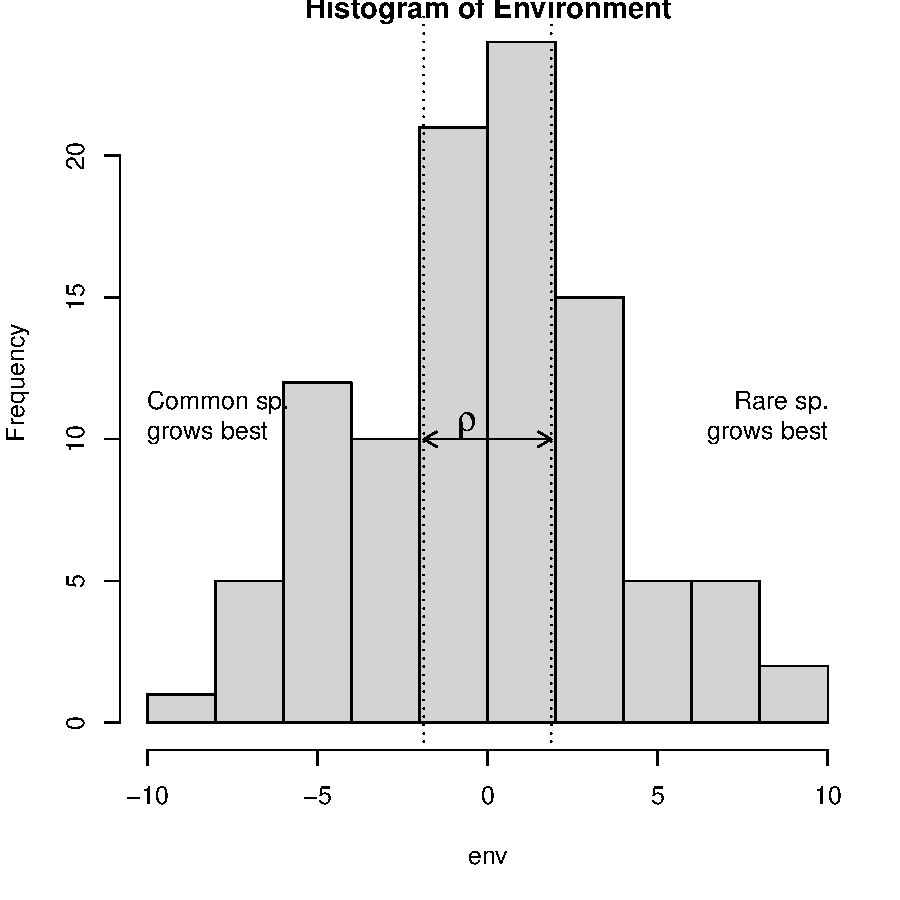
\includegraphics[width=.48\linewidth]{rho} \label{rho}}
  \subfloat[Buffered growth rates]{%
    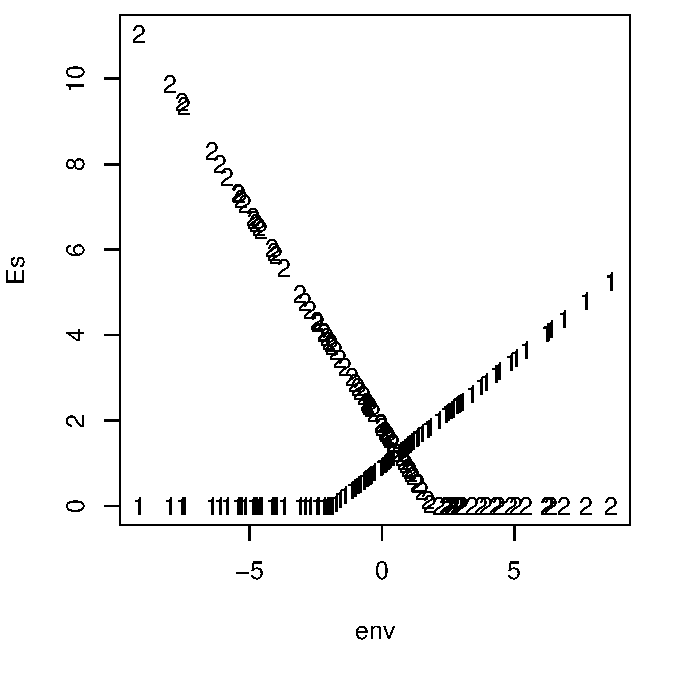
\includegraphics[width=.48\linewidth]{Eenv} \label{Eenv}}
  \caption{Environmental variability, niche overlap ($\rho$), and the resulting buffered population growth rates.}
  \label{fig:rho}
\end{figure}

\medskip \noindent
\begin{boxedminipage}{\linewidth}
  {\footnotesize
\paragraph{Code for a pretty histogram (Fig. \ref{fig:rho})} 
Here we simply create a pretty histogram.
\begin{Schunk}
\begin{Sinput}
> hist.env <- hist(env, col = "lightgray", 
+                  main = "Histogram of Environment")
> abline(v = c(c(-rho, rho)/2), lty = 3)
> arrows(x0 = -rho/2, y0 = mean(hist.env[["counts"]]), x1 = rho/2, 
+     y1 = mean(hist.env[["counts"]]), code = 3, length = 0.1)
> text(0, mean(hist.env[["counts"]]), quote(italic(rho)), adj = c(1.5, 
+     0), cex = 1.5)
> text(min(hist.env[["breaks"]]), mean(hist.env[["counts"]]), 
+     "Common sp.\ngrows best", adj = c(0, 0))
> text(max(hist.env[["breaks"]]), mean(hist.env[["counts"]]), 
+     "Rare sp.\ngrows best", adj = c(1, 0))
\end{Sinput}
\end{Schunk}
}
\end{boxedminipage} \medskip

To quantitfy reproduction as a function of the environment, we will simply let each species growth rate be, in part, the product of its fitness and the environment, with the sign appropriate for each species.
\begin{Schunk}
\begin{Sinput}
> a.rare <- (env + rho/2) * w.rare
> a.comm <- -(env - rho/2) * w.comm
\end{Sinput}
\end{Schunk}
This will allow the rare species to have highest reproduction when the environment variable is above average, and the common species to have high reproduction when the environmental variable is below average. It also allows them to share a zone of overlap, $\rho$, when they can both reproduce (Fig. \ref{rho}).

\paragraph{Buffered population growth}
A key feature of the storage effect is that each species has \emph{buffered population growth}. That is, each species has a life history stage that is very resistant to poor environmental conditions. This allows the population to persist even in really bad times. In some cases, the resistant stage may be a long-lived adult, as with many tree species, or other large-bodied organisms. In other cases, species have very resistant resting stages, such as the eggs of zooplankton \cite{Caceres:1997zv}, or the seeds of annual plants \cite{Facelli:2005kc}. 

To model this buffering effect, we will simply prevent the reproductive rates from falling below zero. (We will, however, create mortality (below) that is independent of the growth rate of each species). Let us impose this constraint of reproduction $\ge 0$ now. 
\begin{Schunk}
\begin{Sinput}
> Es <- matrix(NA, nrow = years, ncol = 2)
> Es[, 1] <- ifelse(a.rare > 0, a.rare, 0)
> Es[, 2] <- ifelse(a.comm > 0, a.comm, 0)
> matplot(t, Es, type = "l", col = 1)
\end{Sinput}
\end{Schunk}
\begin{Schunk}
\begin{Sinput}
> matplot(env, Es, col = 1)
\end{Sinput}
\end{Schunk}
As we said, however, organisms will die. Let us create a variable for community-wide mortality, $\delta$, as if a disturbance kills a constant fraction of the community.
\begin{Schunk}
\begin{Sinput}
> d <- 0.1
\end{Sinput}
\end{Schunk}

\paragraph{Covariance between competition and environment}
\index{covariance|see{environment--competition covariation}}
We also want to assume that species compete for shared, limiting resources. Individuals have negative effects on each other. As a result, the more individuals of all species there are (increasing $N_{total}$), the more negative the total effect is. To account for this, we will stipulate a per capita negative effect $\alpha$ of any individual on any other. Therefore, in good times (high $N_{total}$), the effect of competition increases. In contrast, when times are bad, and $N$ is small, competition is low. This is what Chesson and colleagues mean by \emph{covariation between competition and the environment}. 

Eq. (\ref{eq:storage}) provides a reasonable way to represent the competitve effect $C_{i,t}$. Here we simplify further, and assume that the per capita effect of competition on growth is constant  through time. However, to emphasize that point that one species has higher average fitness, we let the rare species experience greater per capita effects of competition. For our example, let us set $\alpha_{rare}=0.0002, \alpha_{comm}=0.0001$.
\begin{Schunk}
\begin{Sinput}
> alpha <- c(2 * 1e-05, 1e-05)
\end{Sinput}
\end{Schunk}
Thus, these $\alpha$ are the species-specific effects of all individuals on the rare and common species.

\subsubsection{Simulating dynamics}
Finally, we simulate these dynamics. We should create matrices to hold stuff as we simulate each year, for $N$, $C$, and $R$. Unlike $E$, these are simplest to collect as we simulate $N$, year by year.
\begin{Schunk}
\begin{Sinput}
> Ns <- matrix(NA, nrow = years + 1, ncol = 2)
> Cs <- matrix(NA, nrow = years, ncol = 2)
> Rs <- matrix(NA, nrow = years, ncol = 2)
\end{Sinput}
\end{Schunk}
Next we initialize our populations at $t_0$.
\begin{Schunk}
\begin{Sinput}
> Ns[1, ] <- c(1000, 1e+05)
\end{Sinput}
\end{Schunk}

Finally, we run the for-loop
\begin{Schunk}
\begin{Sinput}
> for (i in 1:years) Ns[i + 1, ] <- {
+     juveniles <- sum(exp(Es[i, ]) * Ns[i, ])
+     Cs[i, ] <- alpha * juveniles
+     Rs[i, ] <- exp(Es[i, ] - Cs[i, ])
+     (1 - d) * Ns[i, ] + Rs[i, ] * Ns[i, ]
+ }
\end{Sinput}
\end{Schunk}
and plot the populations.
\begin{Schunk}
\begin{Sinput}
> matplot(c(0, t), Ns, type = "b", log = "y")
\end{Sinput}
\end{Schunk}
\begin{figure}[ht]
  \centering
  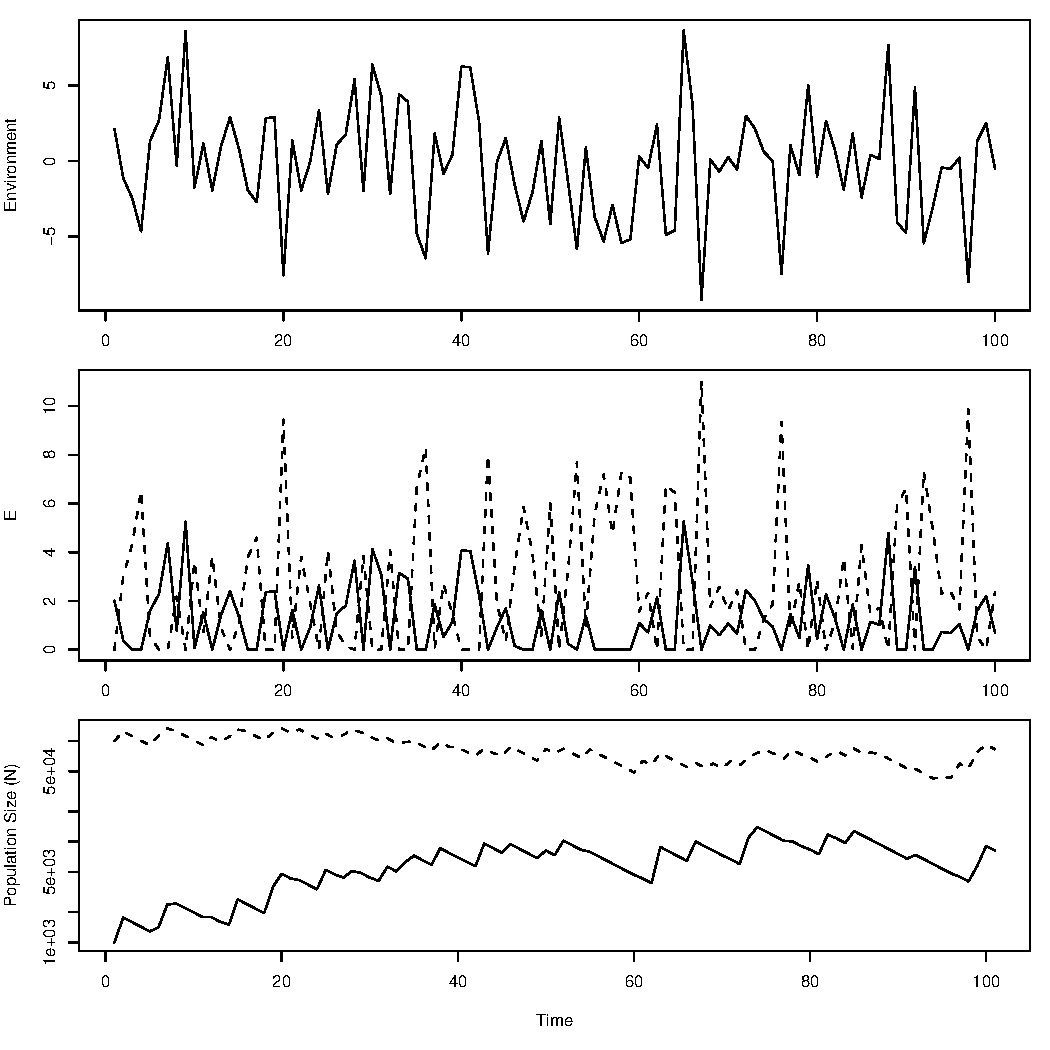
\includegraphics[width=\linewidth]{chessonsim}
  \caption{A simulation of coexistence via the storage effect. $E$ (middle panel) is maximum environment-mediated reproduction, in the absence of competition. See text and Fig. \ref{fig:rho} for more information about species responses to the environment and average fitness.}
  \label{fig:storedyns1}
\end{figure}

\subsubsection{Examining characteristics of the storage effect}
Let us go back and examine a few of the characteristics that we should observe, if the storage effect is operating. First, note that above we showed differential responses to the environment, incomplete niche overlap, and buffered growth (Fig. \ref{fig:rho}). 

Next, we will try to examine the environment-competition covariation. This is not trivial, and papers are written about how to estimate this. For now, recall that in Chapter 3, we began with an examination of negative density-dependence. Here we quantify the magnitude of this negative effect, as our ``effect of competition.'' Let us invent a new value, $\nu$, to measure how much the observed growth rate is affected by large population sizes,
\begin{equation}
  \label{eq:compnu}
  \nu_{i,t} = \log\left(\frac{R_{max}}{R_{i,t}}\right) 
\end{equation}
where $R_{i,t}$ is the observed annual population growth rate, $N_{t+1}/N_t$, for species $i$, and $R_{max}$ is the maximum of these. 

To measure the covariation, we will find first $N_{total,t}$, $R_{i,t}$, and $R_{i,max}$.
\begin{Schunk}
\begin{Sinput}
> Nt1 <- rowSums(Ns)[1:years]
> R.obs <- Ns[-1, ]/Ns[-(years + 1), ]
> Rmax <- apply(R.obs, 2, max)
\end{Sinput}
\end{Schunk}
Now we calculate $\nu_i$, and estimate the covariance.
\begin{Schunk}
\begin{Sinput}
> nu <- log(t(Rmax/t(R.obs)))
> colnames(nu) <- c("nu.rare", "nu.comm")
> var(Nt1, nu)
\end{Sinput}
\begin{Soutput}
     nu.rare nu.comm
[1,]   314.1   763.1
\end{Soutput}
\end{Schunk}
This illustrates that  both populations exhibit positive covariation between the quality of the environment (defined operationally as $N_{total}$) and the intensity of competition.

Last, recall that we stated above that the \index{CV@$CV$|see{coefficent of variation}}$CV$ (\index{coefficent of variation}coefficent of variation) should be greater for rare species than for common species. If we check that for our populations (eliminating the first half of the time series),
\begin{Schunk}
\begin{Sinput}
> apply(Ns[round(years/2):years, ], 2, function(x) sd(x)/mean(x) * 
+     100)
\end{Sinput}
\begin{Soutput}
[1] 29.82 18.14
\end{Soutput}
\end{Schunk}
we see that, indeed, the rare species has a higher $CV$. Examination of the time series (Fig. \ref{fig:storedyns1}) confirms this.

To facilitate playing more games, the function \texttt{chesson} provides an easy wrapper for storage effect simulations (Fig. \ref{fig:chess}). Please try \texttt{?chesson} at the \R prompt.

Here we run the \texttt{chesson} model, and calculate the overlap, $\rho$, for each simulation. 
\begin{Schunk}
\begin{Sinput}
> outA <- chesson(years = 500, specialization = 1, spread = 0.1)
> outB <- chesson(years = 500, specialization = 5, spread = 0.67)
> outA$overlap
\end{Sinput}
\begin{Soutput}
[1] 0.9172
\end{Soutput}
\begin{Sinput}
> outB$overlap
\end{Sinput}
\begin{Soutput}
[1] 0.1234
\end{Soutput}
\end{Schunk}
By specifying greater \index{specialization}specialization and greater spread between the environmental optima of the species pair in the second model, we have reduced \index{niche overlap}niche overlap (Fig. \ref{beta1}). Overlap in this model is the area under both species fitness-independent response curves. Note that large differences in overall fitness can alter effective overlap described by the density-independent reproductive rate, $E_{i,t}$ (Fig. \ref{betaE}).

\begin{Schunk}
\begin{Sinput}
> matplot(outB[["env"]], outB[["Es"]], pch = 1:2, xlim = c(-0.6, 
+     0.6), ylab = "Density-independent Reproduction", xlab = "Environment")
> matplot(outA[["env"]], outA[["Es"]], pch = c(19, 17), add = TRUE)
\end{Sinput}
\end{Schunk}
\begin{figure}[ht]
  \centering
  \subfloat[]{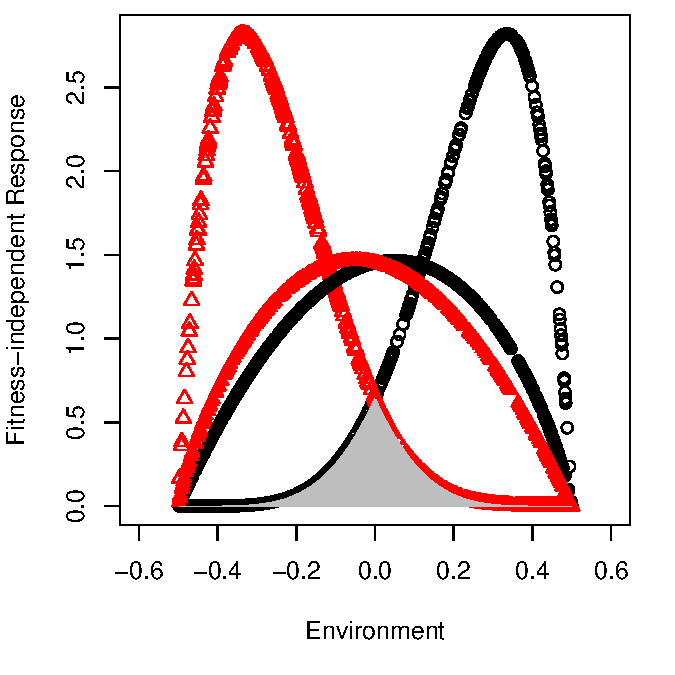
\includegraphics[width=.48\linewidth]{chessonfunc1}\label{beta1}}
  \subfloat[]{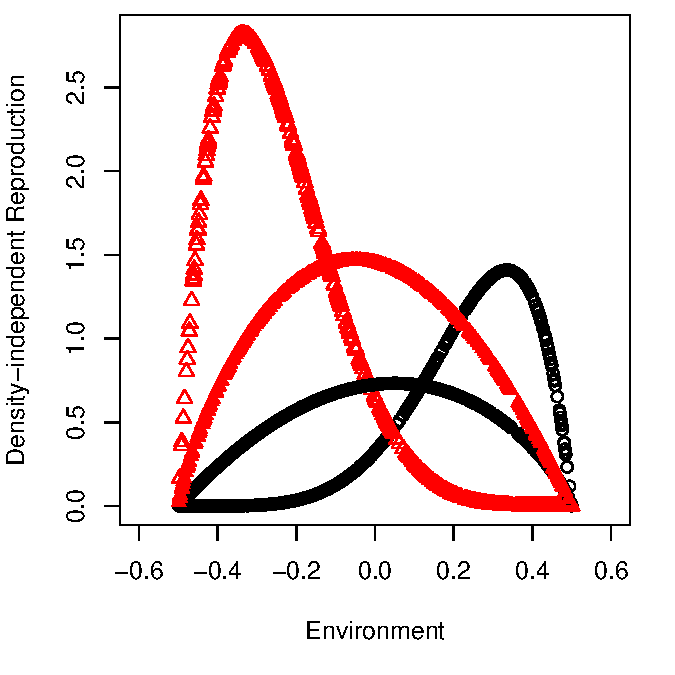
\includegraphics[width=.48\linewidth]{chessonfunc2}\label{betaE}}
  \caption{Species responses to the environment, using the \texttt{chesson} model. Relative to the pair of species represented by solid circles, the pair of species with open symbols shows greater difference between optimal environments (greater \texttt{spread}), and narrower niches (greater \texttt{specialization}).  \subref{beta1} The underlying Beta probability density distributions; the grey \emph{area} under the curves of the more differentiated species is $\rho$, the degree of niche overlap.  \subref{betaE} Density-independent reproduction (the parameter $E_{i,t}$ from eq. \ref{eq:storage}). (grey/red triangles - common species, black circles - rare species; open symbols - highly differentiated species, solid symbols - similar species). See text and help page (?\texttt{chesson}) for more details.}
  \label{fig:chess}
\end{figure}

\section{Summary}
This chapter focused far more than previous chapters on the \emph{biological importance of temporal dynamics}. 
\begin{compactitem}
  \item In the framework of this chapter, the dynamics of succession result from the processes of mortality or disturbance, dispersal, and competitive exclusion.  This framework can be applied over a broad range of spatial and temporal scales. 
    \item Coexistence is possible via tradeoffs between competition, dispersal, and growth rate; the level of disturbance can influence the relative abundances of co-occuring species.
      \item The consequences of habitat destruction depend critically on the mechanisms underlying coexistence. 
        \item The storage effect is an example of \index{temporal niche}temporal niche differentiation. It depends on differential responses to the environment, buffered population growth, and covariation between competition intensity and population size.
\end{compactitem}
 

\section*{Problems}
\addcontentsline{toc}{section}{Problems}

\subsubsection*{Competition, colonization, and the successional niche}
\begin{prob}
  \textbf{Basic interpretation}\\
 (a) Explain each of the paramters $c$, $\alpha$, $\gamma$ and $m$. Explain what each does in the model.\\
\end{prob}
\begin{prob}
  \textbf{Two models in one?}\\
   (a) Given the model of Pacala and Rees, explain which parameters you would manipulate and to what values you would set them to make it a pure competition--colonization model.\\
(b)  Given the model of Pacala and Rees, explain which parameters you would manipulate and to what values you would set them to make it a pure successional niche model.\\
\end{prob}
\begin{prob}
  For each ``pure'' model, explain how transient dynamics at the local scale result in a steady state at the large scale.
\end{prob}
\begin{prob}
  How would you evaluate the relative importance of these two mechanisms in maintaining biodiversity through successional trajectories and at equilibrium?
\end{prob}
\subsubsection*{Storage effect}
\begin{prob}
  Develop a two-species example of the storage effect, in which you manipulate both (i) fitness differences, and (ii) environmental variation. Show how these interact to determine relative abundances of the two species.
\end{prob}
